\documentclass{sig-alternate-05-2015}
\usepackage{graphicx}
\usepackage{subfigure}
\usepackage{times}
\usepackage{url}
\usepackage{cite}
\usepackage{balance}
\newcommand{\bi}{\begin{itemize*}}
\newcommand{\ei}{\end{itemize*}}
\newcommand{\be}{\begin{enumerate*}}
\newcommand{\ee}{\end{enumerate*}}
\newcommand{\tion}[1]{\textsection\ref{sect:#1}}
\newcommand{\fig}[1]{Figure~\ref{fig:#1}}
\newcommand{\eq}[1]{Equation~\ref{eq:#1}}
\usepackage{mathptmx} \usepackage[scaled=.90]{helvet} \usepackage{courier}
\setlength{\parskip}{0pt}
%\setlength{\passp}{0pt}
%\setlength{\headsep}{0pt}
%\setlength{\topskip}{0pt}
%\setlength{\topmargin}{0pt}
%\setlength{\topsep}{0pt}
\setlength{\partopsep}{0pt}
\usepackage{mdwlist}
\usepackage[compact]{titlesec}
\titlespacing{\section}{0pt}{5pt}{*0}
\titlespacing{\subsection}{0pt}{3pt}{*0}
\titlespacing{\subsubsection}{0pt}{2pt}{*0}
\usepackage{balance}

%\titleformat*{\section}{\Large\bfseries}
%\titleformat*{\subsection}{\large\bfseries}
%\titleformat*{\subsubsection}{\bfseries}
%\titleformat*{\paragraph}{\large\bfseries}
%\titleformat*{\subparagraph}{\large\bfseries}
 
\usepackage[svgnames]{xcolor}
\usepackage[framed]{ntheorem}
\usepackage{framed}
\usepackage{tikz}
\usetikzlibrary{shadows}
%\newtheorem{Lesson}{Lesson}
\theoremclass{Lesson}
\theoremstyle{break}

% inner sep=10pt,
\tikzstyle{thmbox} = [rectangle, rounded corners, draw=black,
  fill=Gray!20,  drop shadow={fill=black, opacity=1}]
\newcommand\thmbox[1]{%
  \noindent\begin{tikzpicture}%
  \node [thmbox] (box){%
\begin{minipage}{.94\textwidth}%    
      \vspace{-3mm}#1\vspace{-3mm}%
    \end{minipage}%
  };%
  \end{tikzpicture}}

\let\theoremframecommand\thmbox
\newshadedtheorem{lesson}{Lesson}
 
 
 
% \usepackage{fullpage}
 
\conferenceinfo{BIGDSE}{'16 Austin, Texas USA}

\begin{document}
\pagenumbering{arabic}
\setcopyright{acmcopyright}

\title{The ``BigSE'' Project: Lessons Learned \\from Validating  Industrial Text Mining  }
\numberofauthors{2}
\author{
\alignauthor
Rahul Krishna,  Zhe Yu, \\ Amritanshu Agrawal, Tim Menzies\\ %\titlenote{}\\
       \affaddr{Com Sci, NC State, USA}\\
       \email{\{ rkrish11, zyu9, aagrawa8, tjmenzie\}@ncsu.edu}
% 2nd. author
\alignauthor
Manuel Dominguez,  David Wolf \\%\titlenote{}\\
       \affaddr{LexisNexis, Raleigh, USA}\\
       \email{\{manuel.dominguez, david.wolf\}@lexisnexis.com}
}
\maketitle
 
\begin{abstract}

As businesses become increasingly reliant on big data   analytics, it becomes
increasingly important to {\em test} the choices made within the data miners.
This paper reports   lessons learned from the  {\em BigSE Lab}, an industrial/university
collaboration that augments industrial activity with low-cost testing
of data miners (by  graduate students).  

 BigSE is an experiment in academic/ industrial collaboration.
  Funded by a gift from LexisNexis, BigSE has no specific deliverables. Rather, it is fueled by a research question ``what can
  industry and academia learn from each other?''. Based on open source
  data and tools, the output of this work is (a) more exposure by commercial engineers to state-of-the-art methods and (b) more
  exposure by  students
    to  industrial text mining methods (plus research
  papers that comment on methods on how to improve  those methods).

The results so far are encouraging. Students
at  BigSE Lab have found numerous ``standard'' choices for
text mining that could be replaced by  simpler and less resource intensive methods. Further, that work also found additional text mining choices that could significantly improve the performance of   industrial data miners.
 

{\bf KEYWORDS:}
E-Discovery,  Software Engineering, Testing.

\end{abstract}
% \printccsdesc


\section{Introduction}


Much has been written about the application of data mining
to software engineering. It is now routine to see at major SE
conferences that a third (or more) of the papers used data miners
to augment their analysis.
Clearly, data mining has much to teach software engineering, but what about the other way around? What can software engineers teach
data mining? What are the lessons learned from decades of SE that
can improve data mining?


In 1975, Fred Brooks noted that half the effort 
of a software project is spent in {\em testing}. In an update
to that book~\cite{Brooks95}, written twenty years later, Brooks still
asserted that testing remains a large task within any project.
Accordingly, we should expect that when industrial data mining
providers ship analytic tools, they should conduct extensive
testing of those tools prior to release.


Some parts of commercial data mining tools are thoroughly tested prior to
release (e.g. distributing tasks across
a CPU farm or array of disk storage). However, other parts
may not be so extensively explored. For example, 
LexisNexis  is an international commercial company that offers
Big Data solutions to clients. LexisNexis has
invested time writing support and mining tools to assist with {\em E-discovery} (discussed
in the next section).  
When LexisNexis ships E-Discovery products, those products contain
numerous text mining {\em operators} to handle (for example)
tokenization, featurization, normalization, classification, etc. 
Once a set of operators offers promising results,
standard practice is to configure the text mining tool
with those operators, then ship the resulting product.

LexisNexis contacted NcState with the question of ``how can
we validate if the operators we select for text mining are 
satisfactory?''. This is a tricky problem in a commercial
environment since an extensive exploration of  data mining operators for
tokenization, featurization, normalization, classification, etc.
is a massive task. Having run such studies for many years~\cite{menzies2014sharing},
we can assert that this is mostly a trial-and-error process
with a high percentage of errors. Commercial practitioners, responding to market pressures, may not be willing to explore this  space of option
since the large numbers of negative results are not consistent
with an approach that quickly delivers incremental value to the market:
\bi
\item
The advantage
of this approach is that, using it,  commercial companies can maintain or extend their revenue stream.
\item
That said, it discourages extensive experimentation, and doesn't reward  long sequences of negative results as data scientists try various options.
\ei

The trials and errors associated with exploring text mining operators
are more suited to a research environment where persistent effort, with only occasional positive results, is more acceptable. Hence,
LexisNexis and NcState jointly created the {\em BigSE Lab}  where
university graduate students explore    the space of text mining
operators proposed by 
industrial engineers.  Funded by a gift from LexisNexis, the project has no specific deliverables. Rather, it is fueled by a research question ``what can
  industry and academia learn from each other''. Based on open source
  data and tools, the output of this work is (a) more exposure by commercial engineers to state-of-the-art methods and (b) more
  exposure by graduate students
    to more industrial text mining methods (plus research
  papers that comment on methods on how to improve  those methods).





This paper documents the lessons learned from the BigSE project. 
These lessons divide into {\em process} insights (comments
on methods for organizing this kind of collaboration) and {\em technical
insights} (comments on different operators for text mining).
 
 
  
   


\section{About the Domain: E-Discovery}

The specific  task explored in this work was {\em E-Discovery}.
E-Discovery is part of  civil litigation where one party (the producing party), offers up   materials which are pertinent to a  legal case. The producing party makes the materials available to a requesting party.
Upon reception of a request, it is the duty of the producing party to make an inquiry to find all reasonably relevant materials in their possession and turn them over to the requesting party.
In the case of a modern company, this may mean searching through 
millions emails to find (say) $100$ emails that are most relevant to the case at hand.
  
This process is extensively monitored by both sides involved in the litigation,
as well as the judges overseeing the process. Companies can be heavily sanctioned if
they fail to conduct a reasonable search in good faith, or if they do not respond in a timely
manner\footnote{\url{https://www.law.cornell.edu/rules/frcp/rule_26}}. If the producing party is perceived to be working in bad faith during this process, then this
can result in court sanctions. Hence, there is much commercial interest in 
E-Discovery tools that  are thorough and discourage over-use, misuse,   or abuse of procedural tools that increase cost and result in delay.

\begin{comment}
TIMM: COVERED!
Manny: "burying the other side with paper" or "over producing" is a rare thing these days.  See the FRCP Rule 1 and  Committee note:  
Rule 1 is amended to emphasize that just as the court should construe and administer these rules to secure the just, speedy, and inexpensive determination of every action, so the parties share the responsibility to employ the rules in the same way. Most lawyers and parties cooperate to achieve these ends. But discussions of ways to improve the administration of civil justice regularly include pleas to discourage over-use, misuse, and abuse of procedural tools that increase cost and result in delay. Effective advocacy is consistent with — and indeed depends upon — cooperative and proportional use of procedure.
\end{comment}

Initially, document discovery was a mostly manual process conducted by teams of attorneys. 
Team members would laboriously read through all the documents, marking them as important or otherwise with tags based on the document's relevance to the request. This method of search is now known as \textit{linear review}. 
Baron et al.~\cite{baron2006trec} report that the review rates for different topics at the TREC 2006 Legal Track ranged from 12.3 to 67.5 documents per hour, and averaging 24.7. In 2007, the average review rate was around 20 documents per hour, and around 21.5 per hour in 2008~\cite{oard08}. Roitblat et al.~\cite{roitblat} reported that for a large-scale review, 225 attorneys were required to each work nearly 2,000 hours to review 1.6 million documents, at a rate of 14.8 documents per hour. Borden~\cite{borden} cites a review of ``fairly technical'' documents running at the rate of 45 documents per hour, and states 50 to 60 documents per hour as the ``e-discovery industry average.''

The time required for linear  review depended on several factors relating to document
collection, requests, and reviewer time. The typical review rate was a few minutes per document. As is to be expected, with the growth in size of the collection, such a review process becomes more and more impractical. To remedy this issue a higher degree of automation is required.
The  process of E-Discovery is summarized  by a widely-cited EDRM Reference Model\footnote{http://www.edrm.net/resources/edrm-stages-explained}.  Starting from ``Information management'', where the intent is to incorporate all the information processing that is required by the organization before the e-discovery process starts, to ``Presentation'' which is
the part of the process that  prepares   depositions, etc. 

\begin{comment}
TM: COVERED!
Manny: "``Presentation'' on the right, which involves the production of the discovered materials to support a legal analysis." Analysis and Presentation are not really related to production.  Usually opposing counsel receives a production from the defendant. Then they use tools to analyze the data they received and to "trial presentation software" (PowerPoint as a simple example) to prepare for depositions, etc.  See EDRM stages for more information:
http://www.edrm.net/projects/metrics/utbms
It's also important to note that the EDRM is not a linear process that starts on the left and goes to the right (it rarely does).  That's why the model has back arrows in addition to forward arrows.
See the 2014 EDRM model:  http://www.edrm.net/resources/edrm-diagrams-a-history
\end{comment}


The LexisNexis experience is that
``Document search'' represents 60 to 80\% of the total  cost. Hence, this
work focused on improving that search capability. 
 
 


\section{Process Lessons}
This reviews BigSE's  infrastructure
and week-to-week working.  Some of the lessons listed in this section will not
surprise those already familiar with Big  Data projects. We present
them nevertheless since, if the
reader wants to propose something like BigSE to their organization, 
then  their management might find the process lessons of
this section
most relevant.


\subsection{Hardware}

Modern Big Data infrastructures make it possible to offer a faster series of conclusions to industrial partners.
For example, using BigData tools,
NcState was able to maintain the interest
of LexisNexis engineers with a continual stream of
weekly innovations and other results. BigSE students run their experiments on the   NcState
High Performance Computing facility (HPC is a network of 10,000 machines with 2 to 8 cores on each).
A standard run for us is a 25 times repeat cross-validation experiment where data
5 variants of a learner are run over 25 data sets. Depending on the size of the data and the speed of the learner, such a run can take hours to days to 
terminate on a single machine.  However, on HPC, that same run terminate in times
as short as 30 minutes. Note that it took a few
weeks of script tweaking before we take full   advantage
of HPC but that was time well spent since it meant we could:
\begin{lesson}
Use Big Data     to generate
more conclusions, sooner.
\end{lesson}  
\begin{figure}
\includegraphics[width=3.5in]{fig/example.png}
\caption{Example Stackoverflow.com data used in this work.}\label{fig:example}
\end{figure}
\subsection{Domain Sampling Materials}
At the start of the project, LexisNexis spent some effort
building and presenting training materials to 
introduce NcState to their business domains.

Those materials were of two forms. Firstly,
at the first four weekly 
meetings, LexisNexis presented slides 
describing the business
domain within which the text mining was to occur. 
These briefings were important in learning what
mattered, and what did not matter, to the industrial
client.
\begin{lesson}
In an industrial/academic
relationship, it will take
some time for the industrial
partner to explain the details
of their business to an academic partner. 
\end{lesson}  

The second form of materials that was important
to this project was a  ``mock'' data generator.
This ``mock'', built by LexisNexis, generated   data  
representative of the kinds of data seen in industrial practice. 
Given a random number seed, this ``mock'' pulled
data from Stackoverflow.com (e.g. see \fig{example})
and built
a data set  containing the attribute
and class distributions seen in current LexisNexis E-Discovery work.

The importance of the ``mock'' was three-fold. Firstly, it gave NcState ready access to large
numbers of non-confidential data sets. Secondly, when we reported results, it gave LexisNexis confidence
our methods would work on their kind of data.
Thirdly, the LexisNexis ``mock'' taught  NcState about the unique features of
the problems faced during E-Discovery.
Much of the literature on text mining Stackoverflow.com
assumes ``tag-level'' while the data more relevant to E-Discovery
is ``site-level'', which we characterize as follows:
\bi
\item
{\bf Tag-level}:   Each data set contains  thousands of posts. The title and body of the posts are concatenated to form the independent variables for classification. The first tag for the posts is treated as the class of the post. In each data set, one specific tag is selected as the ``relevant'' class and all other tags are considered as ``irrelevant'' class.
\item
{\bf Site-level}: generated from the LexisNexis ``mock'', 
which produces a two-class data set comprising 20000 threads, where
 ``relevant''
examples from one specific sub-site were 2 to 6\% of the data. The task of site-level prediction is to predict which sub-site a test example belongs to, instead of tag.
\ei
The site-level/tag-level distinction is important since much of
the text mining literature on Stackoverflow.com is
aimed at tag-level tasks~\cite{moharanatag,stanley2013predicting,kuo2011word}. For example, Clayton and Byrne, 2013 \cite{stanley2013predicting} have worked on StackOverflow tag prediction and developed an ACT-R inspired Bayesian probabilistic model. This approach achieves a $65\%$ of accuracy by choosing the tag that has the highest log odds of being correct, given the tag's prior log odds of occurrence and adjusting for the log likelihood ratio of the words in the post being associated with the tag.
For another example,  see also Kuo, 2011 \cite{kuo2011word}'s work on predicting the next word in a corpus-- which is an interesting
task but not relevant to E-Discovery.


In the following, we show that focusing on site-level,
lets us find better choices for text mining this particular
kinds of data. Hence:
\begin{lesson}
Text mining methods should be tuned to specifics
of the data set used in a particular context.
\end{lesson}  
\begin{lesson}
After sorting out the CPU farm, the next  important task is to
build a ``mock''   generator for data that is representative of the specific
target domain.
\end{lesson} 



\subsection{Other Management Details}

\subsubsection{Nondisclosure Agreement}

All students and faculty involved in BigSE
 sign non-disclosure agreements with LexisNexis. The particular NDA used
 here was not particularly restrictive. Researchers at NcState agreed not to share confidential
 information gained from LexisNexis as well as being somewhat circumspect in their publications
 (e.g. showing LexisNexis engineers drafts of any paper and asking for comments and/or
 corrections).  In return, NcState agreed to document all their analysis of   publicly
 available data sets and tools, shared with LexisNexis engineers in private Github repositories.  The ease
 with which these NDAs were developed taught us that:
 \begin{lesson}
Corporate confidentiality is an important
concern, but it does not need  to  stifle
industry/research interactions regarding Big Data.
\end{lesson} 
\begin{lesson}
Use of open source tools and data aids collaborative interactions
between industry and academia.
\end{lesson}
 \subsubsection{Use of Github}
The Github repositories proved useful in several  ways.
Firstly,
 LexisNexis  engineers have immediate and ready access to 
 any interesting methods and/or findings created by NcState. 
Secondly,
rather than wasting time writing PowerPoint slides, NcState students could
report their results using the Markdown tools within the Github issue
report systems.
Thirdly, using Github, LexisNexis developers could monitor and provide
quick feedback on the NcState code and issues,
as they arose.
Lastly, and perhaps more importantly for building
a trusting relationship,
LexisNexis could see consistent effort on the part of NcState. SeLAB members
are urged to do all their planning and coding and task management in Github.
This gives LexisNexis an accurate appreciate for all the work conducted
by the graduate students.
 \begin{lesson}
Github tremendously simplifies  industry/ academia communication for projects
that make extensive use of prototyping.
\end{lesson}

 \subsubsection{Staffing and Training}
To start-up the lab  BigSE, LexisNexis funded several graduate students for one year. Also,
LexisNexis engineers gave talks at NcState graduate recruitment days (and to
the graduate seminar series). From those talks, several other non-paid graduate students
joined the project as part of their research hours subjects. In all, BigSE is
now staffed by six graduate Ph.D. students who sit in adjacent cubicles and who
 share their coding tools and tricks. 

Newcomers to BigSE are given analysis tasks
 that the team has previously completed and asked to reproduce the results or challenge them. For
 that initial study, they have access to all prior code written by the team
 and their challenge is to understand the parts and assemble them into a working
 whole. 
 
  LexisNexis and NcState meet each week to present and review the results. That meeting includes
a round robin session where each graduate student is asked to show some results,
or say ``pass''. This session imposes some competetive pressure on the students to achieve
results in order to ``show off'' in front of their peers and in front of the
LexisNexis engineers. Not every student is expected to have something to show each week,
but it becomes abundantly  clear within the overall team if some student is ``passing'' all
the time.

 While our  students have a steep learning curve in their
 first two months, by month three they are typically generating results that surprise and interest LexisNexis.
 Hence, with the proviso that  newcomers can be immersed in an environment
 with  more experienced people:
  \begin{lesson}
With the right support structures, novice
Big Data graduate students
can become productive in two to three months.
\end{lesson}
 \subsubsection{Schedule and Tasks}
As to specific tasks, graduate students are assigned a mix of projects. Some are very short-term (e.g a one week
study on the merits of TF*IDF vs term frequency) and some are more medium to long-term
that can take weeks to months (e.g. literature reviews on entity recognition or
active learning experiments). 

Initially, to build trust between LexisNexis and NcState, the focus of the work was on very
short term projects (weekly incremental reports). Now, the focus has changed and
LexisNexis is prepared to discuss longer-term projects that deliver incremental value, that may yet take months to complete.  Hence we recommend:
\begin{lesson}
Initially, build trust with   short-term goals,
then expand   later.
\end{lesson}
\subsubsection{Preparing for  ``Critical Audits''}
This ``portfolio'' approach  that combines short low-risk tasks with longer high-risk tasks is useful management trick for speculative projects.
In commercial endeavors, every so often, projects receive a critical  ``audit''  where engineers have to
occasionally prove their worth to a (perhaps) critical audience that is eager  to cut
expenses.  So far,
there have been no critical audits of the BigSE project, but it is always
best to be prepared.
Ensuring a continual supply of conclusions (from the short-term projects),
is one way to increase the odds of surviving the critical audit. Hence we advise that:
\begin{lesson}
It is useful to run a mix of short and long term projects.
\end{lesson}
 
  


\section{Technical Lessons}
\label{sect:Method}
The experiments performed at BigSE are many and varied and constantly
changing. So far, we have focused on 
methods to improve classification, active learning, and entity
recognition. 

In order to report within
the seven page limit of this paper, we focus here on the
classification work. 
Note that the following results are not a claim that the
best way to do all text mining is via the methods
championed below. Rather, we say that for the specific site-level
problem explored by LexisNexis for the E-Discovery work,
the following choices have been found to be useful. For other
kinds of data, we would recommend further study to find
the results that work best for those other kinds of data.


\begin{comment}
\subsection{Improving over the baseline}
Prior to BigSE,
the baseline LexisNexis text miner for site-level data was:
\bi
\item Tokenize with the {\em stemming} and {\em stop words};
\item Featurize with {\em term frequencies};
\item Normalize using {\em L2 normalization};
\item Dimensionality reduction with the {\em hashing trick};
\item Classification using SVM with a linear kernel.
\ei
(All the above terms in {\em italics} are explained below.)

The above list is one point within a very large space of options.
The text mining literature offers many alternatives to the above:
\bi
\item  Some method to handle class imbalance
\item Different choices for the items listed above
such as TF*IDF for the featurization or SVMs with different kernels.
\ei
The general approach in BigSE is to explore other options
than those listed above;  i.e. given the choices made by LexisNexis'
engineers in their text mining, change {\em one} choice
and see what can be improved.  
\end{comment}
\subsection{Performance Metrics}

%\textbf{RQ2} What is the proper performance metric for this task?

There are two contradictory goals that should be achieved according to our task: 

\textbf{a) Precision} ($p$) since all the documents being predicted as 'related' should be examined by human efforts, a high precision can greatly reduce the cost of this examination.

\textbf{b) Recall} ($r$) a high recall can reduce the number of 'related' documents that we failed to retrieve.

For the purpose of studying both precision and recall, we use:
 \mbox{$F_{1}=  2pr/(p+r)$}
as  our  performance metric.

\subsection{Standard Experiment}
%-----
%
Starting with  LexisNexis' default
settings to their text miners (stemming and stop words removal for tokenizer, term frequency for featurization, hashing trick for dimensionality reduction, L2 normalization on rows for normalization, linear SVM for classifier), we
 modified one option at a time (e.g. swapped the hashing trick for Tf*idf).
Different options in a single process (e.g. hashing trick and TF-IDF selection in dimensionality reduction) were compared in each experiment with 5 by 5 cross-validation ($20\%$ as training sample and $80\%$ as testing sample since in real tasks, the training sample is always less). 
This rig was applied to 10 tag-level problems and 15 site-level problems (using an SVM
with a linear kernel as the classifier).

\subsection{Comment on External Validity}

% Move up

There are several validity threats to the design of this study: 

\textbf{a)} The above experiments show results from a
limited number of text mining methods.
The space of known text mining methods is truly vast
and the following studies represent just a small portion of the total space.

 
\textbf{b)} All the above used data that we have characterized as tag-level or site-level samples
from posts in Stackoverflow.com. For other kinds of data, we recommend repeating this
analysis to find the right text mining methods for that kind of data.

Due to these threats to external validity,   we make no presumption that the following conclusions work best   for all text mining applications. We only assert that the following   work better some
alternatives 
  in our domain.   
  
That said, we   assert that the following is   externally
valid:
\begin{lesson}
Commercial organizations can outsource
at least some of their 
their validation work to university partners.
\end{lesson}
Further, within that validation
process:
\begin{lesson}
The university partners can sometimes find
better choices that those currently employed by the commercial
organization (e.g. see the SMOTE results, below).
\end{lesson}



\subsection{  Results}
The results are 
presented in  Figure \ref{fig:all}.
Three interesting results in those plots are listed below.

{\em 1. Performance deltas:}  In Figure \ref{fig:all}, the
tag-level problems are shown on the left and the site-level problems are
shown on the right.  The results show a low valley on the left and higher plateau on the right; i.e.   methods that work well for site-level
do not work well for tag-level. This result underlines Lesson 3\&4 on the 
  importantance of testing via   data that is particular to specific domains.
 
{\em 2. Low IQR:} In  Figure \ref{fig:all},
the solid lines at the top show the median (50th percent) value
and the dotted lines at bottom show the IQR (the inter-quartile range calculated from the (75th-25th) percentile). Note that, usually, the dotted lines are close
to zero; i.e. the variance in our conclusions across multiple samples is mostly
very low. Hence:
\begin{lesson}
The performance variance is small enough to make  definitive statements about what methods work best for  site-level problems.
\end{lesson}

{\em 3. Blurred results:} Ig is difficult to distinguish between   some the  results since, looking at Figure \ref{fig:all} (a) and (b) and (c),   the overall benefit of certain treatments is marginal.
That is:
\begin{lesson}
Not all standard text mining methods are  powerful or useful.
\end{lesson}

The rest of this section discusses more specific results.


\label{sect:Experiment}

\subsubsection{Tokenization}

Tokenization is the very first step in natural language processing. It removes the spirit of symbols by identifying the most basic units which need not to be decomposed in the subsequent processing \cite{webster1992tokenization}. 
\textbf{Shingling} introduces phrases as unit token. A word-based $w$-grams shingling captures contiguous sequences of words as unit tokens and each unit token has $w$ words \cite{chang2009using}. Bigram and trigram shingles uses w=2 and w=3-grams, respectively.
\textbf{Stemming and stop words removal} combines words that have same meaning and removes  very frequently used words. An example of stemming and stop words removal 
would be to convert ``i want to eat apple since i like eating apples'' to
``want eat apple since like eat apple''.
While stemming and stop words are considered  an effective way to improve the text classification performance \cite{yang1997comparative},  some contradictory evidences deprecates these techniques~\cite{moharanatag,stanley2013predicting}. 


% \begin{figure}[ht]
%   \includegraphics[width=\linewidth]{./fig/pre.eps}
%   \caption{Tokenization}
%   \label{fig:pre}
% \end{figure}

 
The   cost of these tokenizers is very low (each can be completed in a simple pass
through the data) but their observed   benefit is small.
As shown in Figure \ref{fig:pre}, the average improvement of stemming and stop words removal in median value is 1\% on tag-level data  and 6\% on site-level  data sets.
Note that  deltas are very close to the IQRs of 3\%,4\% for tag-level,site-level (respectively).  Hence:
\begin{lesson}
Despite their prominence in the literature, the benefit of stemming and stop words
and shingling for our data sets  is minimal.
\end{lesson}


\begin{figure*}
    \centering
    \subfigure[Tokenization]
    {
        \includegraphics[width=0.48\linewidth]{./fig/pre.eps}
        \label{fig:pre}
    }
    \quad
    \subfigure[Featurization]
    {
        \includegraphics[width=0.48\linewidth]{./fig/fea.eps}
        \label{fig:fea}
    }
    \quad
    \subfigure[Number of Features]
    {
        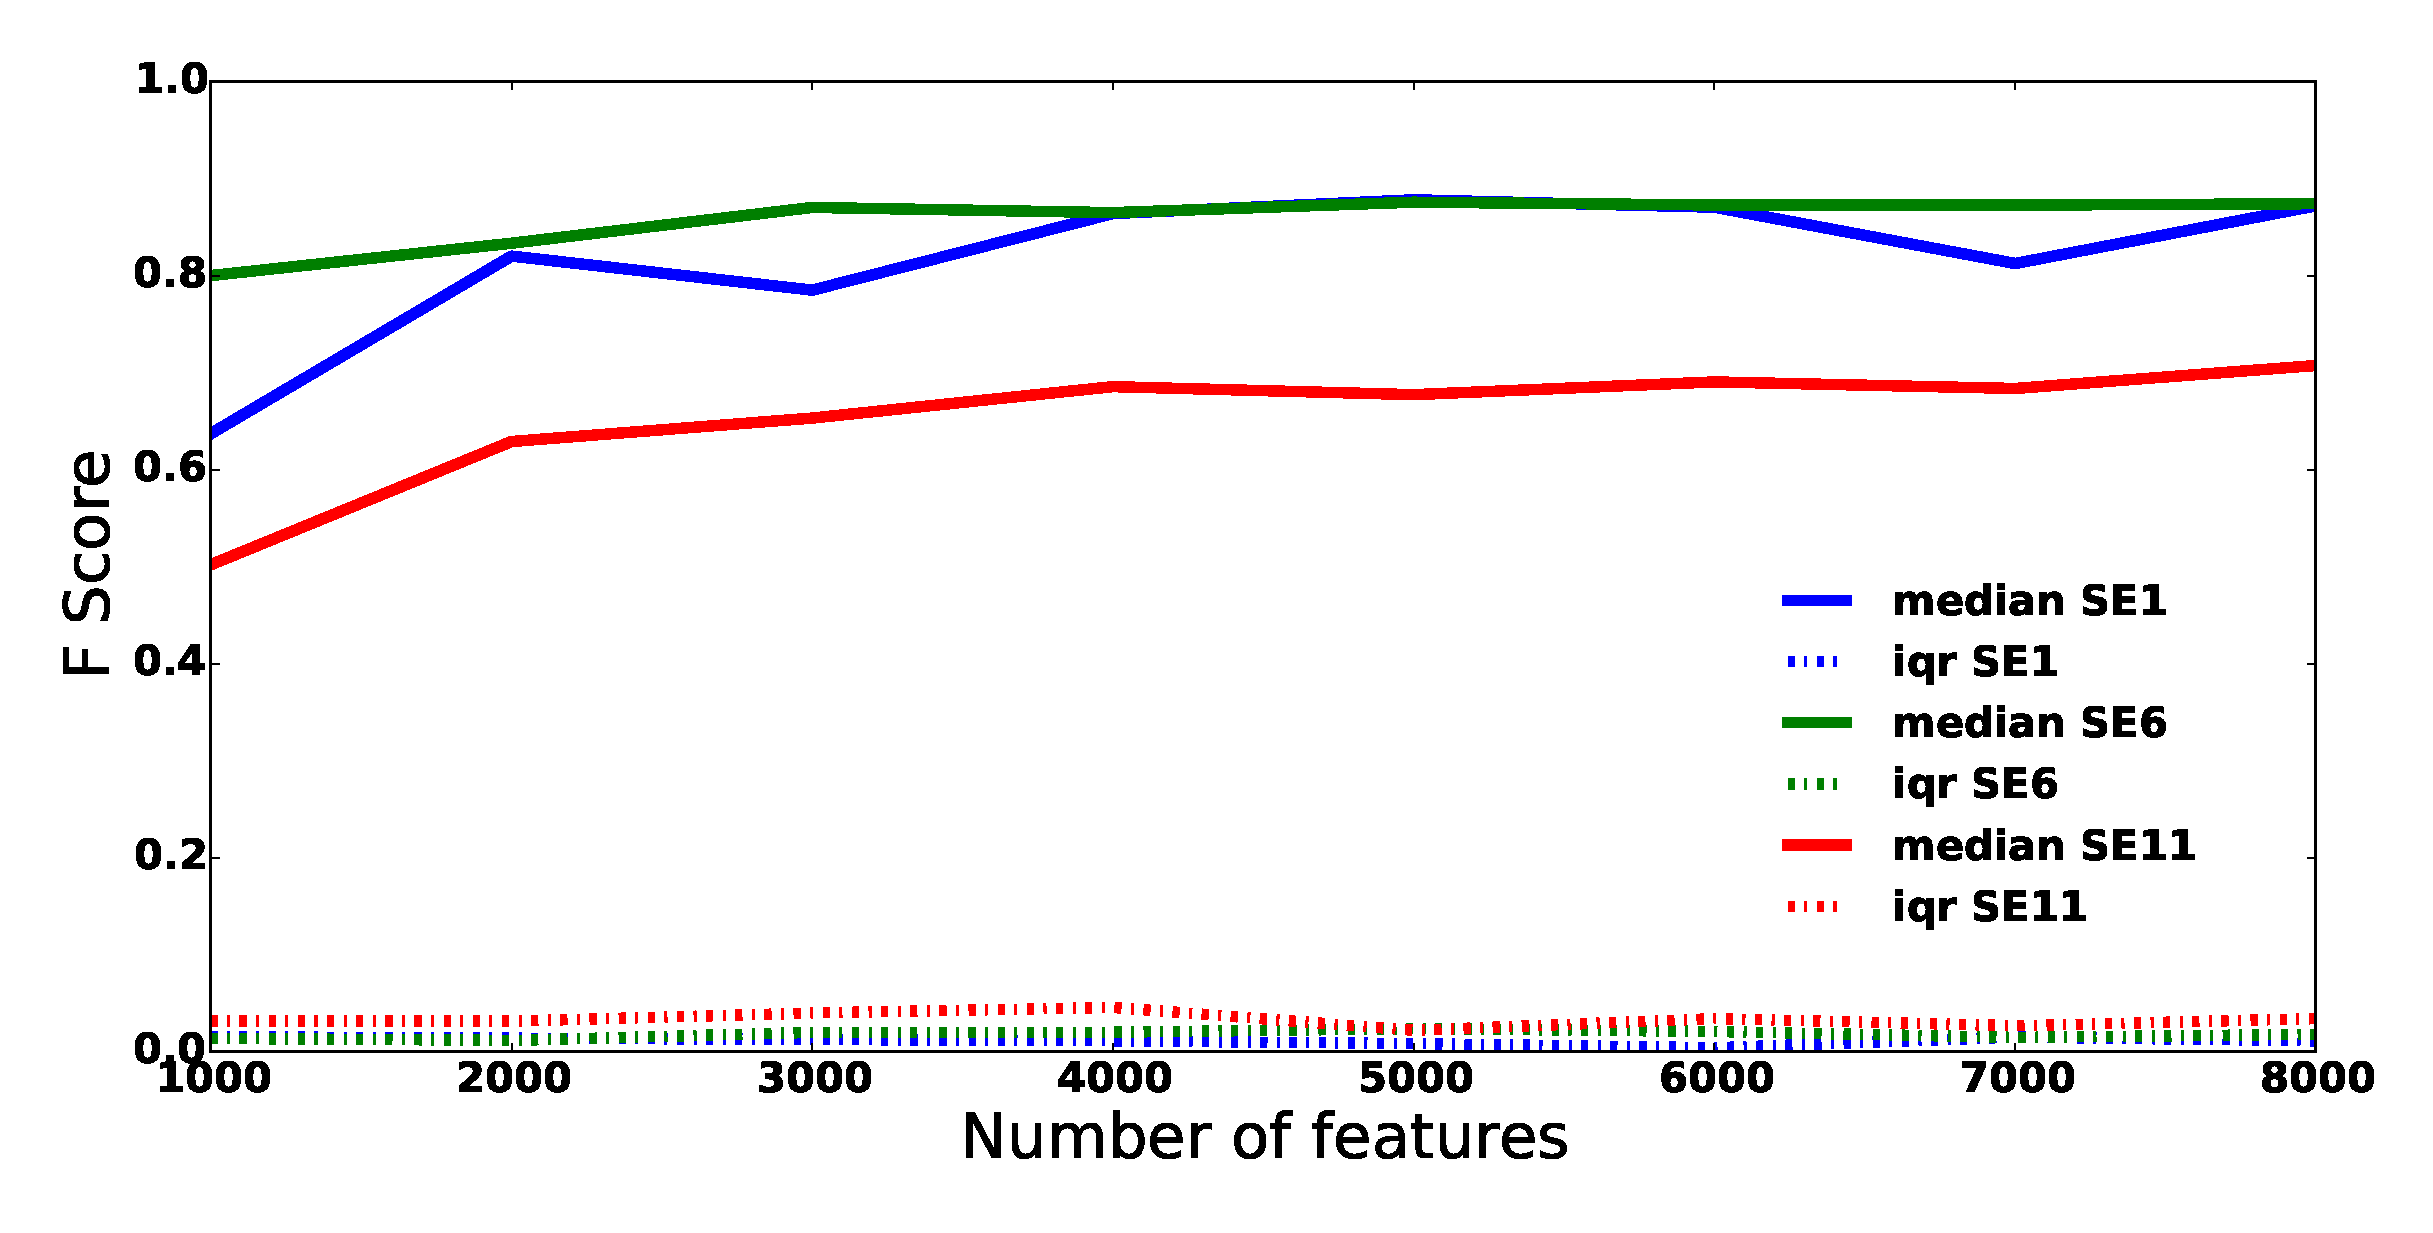
\includegraphics[width=0.48\linewidth]{./fig/fea_num.eps}
        \label{fig:fea_num}
    }
    \quad
    \subfigure[Dimensionality Reduction]
    {
        \includegraphics[width=0.48\linewidth]{./fig/sel.eps}
        \label{fig:sel}
    }
    \quad
    \subfigure[Normalization]
    {
        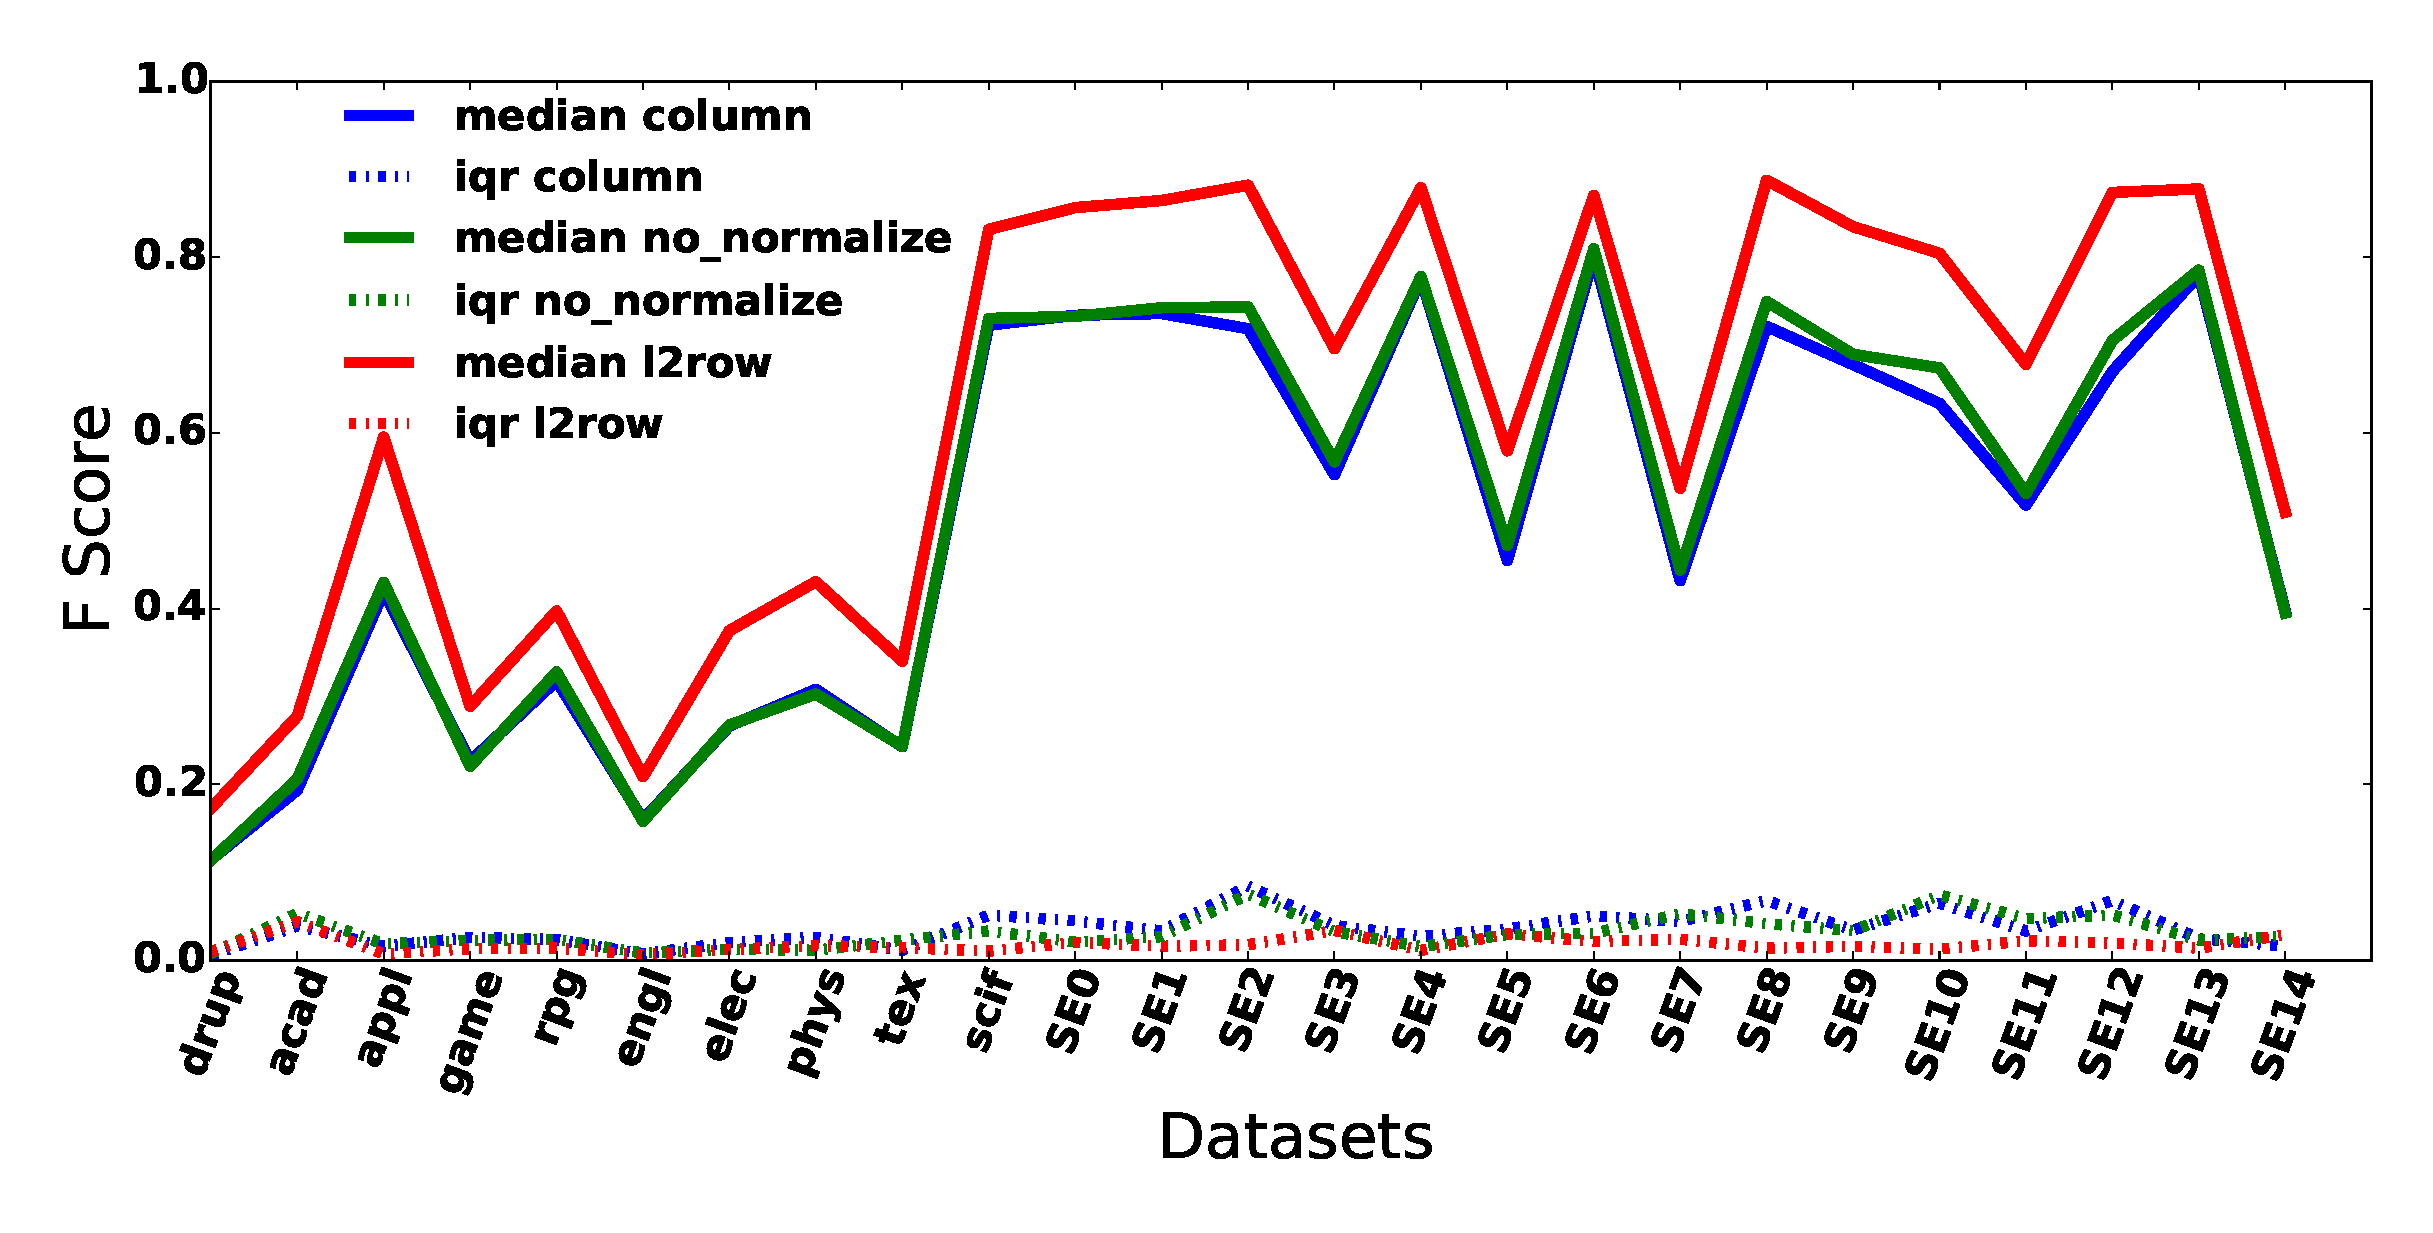
\includegraphics[width=0.48\linewidth]{./fig/norm.eps}
        \label{fig:norm}
    }
    \quad
    \subfigure[Data Balancing]
    {
        \includegraphics[width=0.48\linewidth]{./fig/balance.eps}
        \label{fig:balance}
    }
    \quad
    \subfigure[Classifiers]
    {
        \includegraphics[width=0.48\linewidth]{./fig/algms1.eps}
        \label{fig:algms1}
    }
    \quad
    \subfigure[SVM Kernels]
    {
        \includegraphics[width=0.48\linewidth]{./fig/algms2.eps}
        \label{fig:algms2}
    }
    \caption{Results seen in multiple 5*5 cross-validation experiments. Unless
    otherwise specified, the learner here is an SVM with a linear kernel.
    In all these plots, {\em higher} lines mean {\em better} performance.
    Within each plot,  the solid lines (at top) are median scores and 
    the dashed lines (at bottom) are inter-quartile ranges (75th-25th percentile). Also, except for Figure \ref{fig:fea_num} ten left-hand-side data sets are tag-level while the remaining are site-level data sets generated from
    our ``mock'' data generator.
    }
    \label{fig:all}
\end{figure*}


\subsubsection{Featurization}

Featurization is the process which transforms the tokens of each document into a vector of weights of each unique token, which can be used to train the classifier~\cite{manning1999foundations}. 
\textbf{Term frequency}, also known as word count \cite{manning1999foundations}, would convert ``want eat apple since like eat apple'' to
{\em \{eat: 2,\, apple: 2,\, want: 1,\, since: 1,\,like: 1\}}.
\textbf{Tf-idf weight }calculates not only the word count, but also the number of documents each token appears, calculated as follows:

\begin{equation}\label{eq:tfidf}
\mathit{tfidf}(t, d) = |t  \in d| \cdot  log\left(\frac{|D|}{|d\in D: t\in d|}\right)
\end{equation}
where $D,T$ are all documents and tokens and $t\in T,d\in D$.
The intuition behind  Tf-idf   is that the more frequent a token appears and the less documents it appears in, the more important it is. Tf-idf  is  a popular feature for text categorization\cite{caropreso2001learner,moharanatag}. 


% \begin{figure}[ht]
%   \includegraphics[width=\linewidth]{./fig/fea.eps}
%   \caption{Term frequency vs tf-idf weight}
%   \label{fig:fea}
% \end{figure}

 
As shown in Figure \ref{fig:fea}, term frequency performs no worse     than tf-idf weight.  Hence:
\begin{lesson}
Despite its   prominence in the literature, the added value of Tf*idf for our
data sets is minimal.
\end{lesson}

\subsubsection{Dimensionality Reduction}

%\begin{figure}[!t]
 % 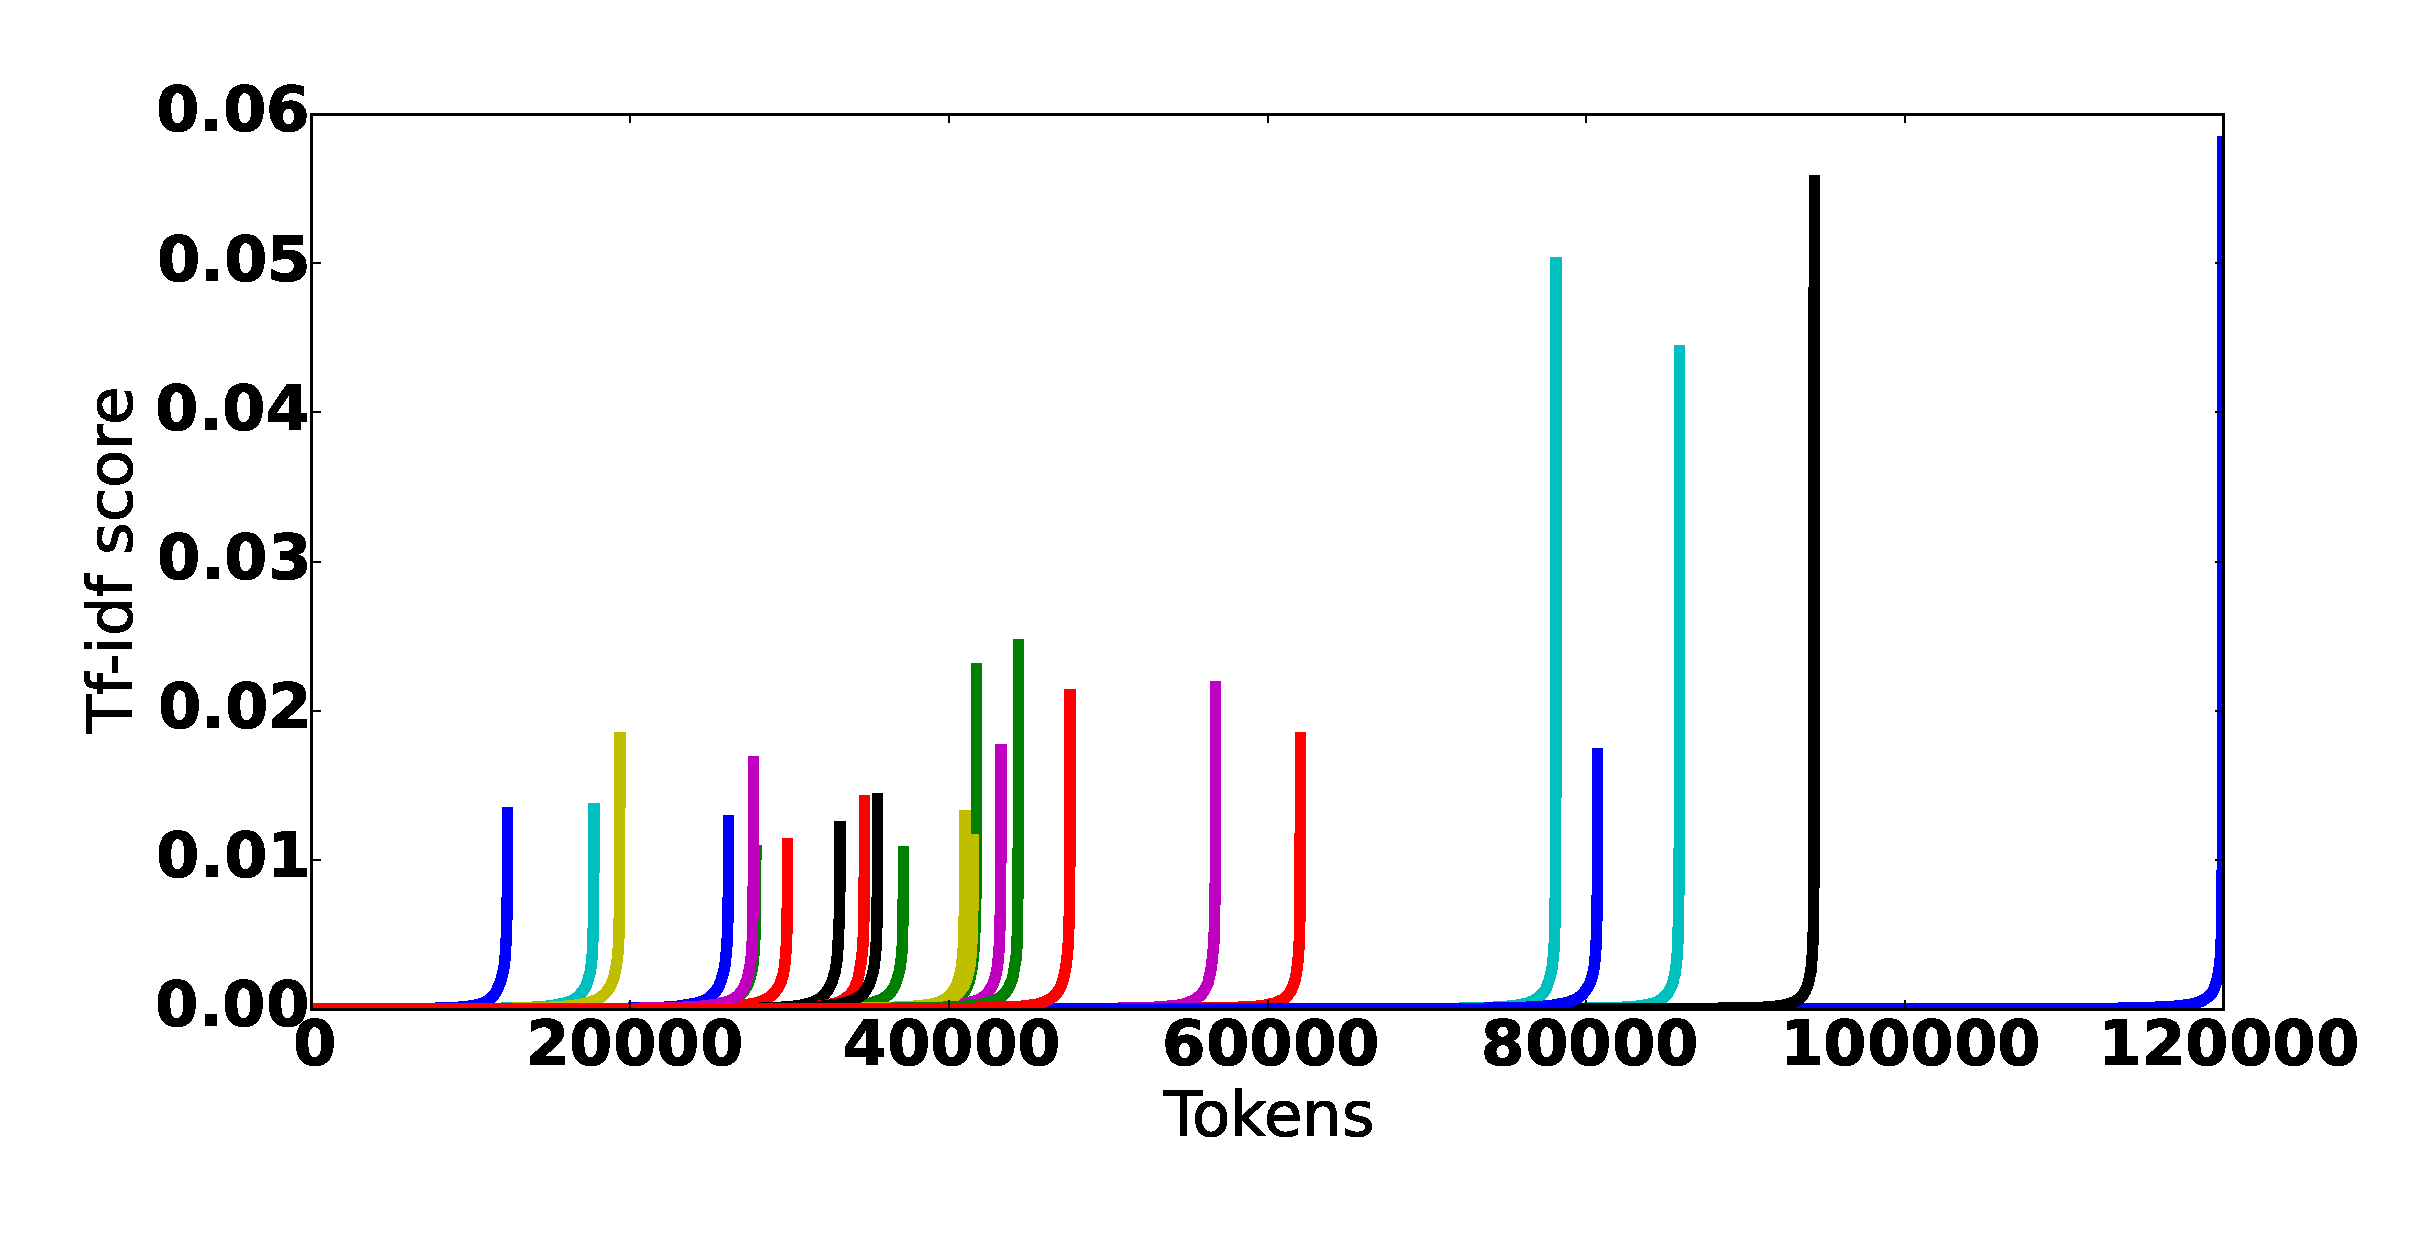
\includegraphics[width=\linewidth]{./fig/tokens.eps}
  %%\caption{Information of tokens}
 % \label{fig:tokens}
%\end{figure}

Dealing with the tables of data containing all the words in English, would mean processing a very large number of columns. A useful method for removing noise and reducing the 
memory costs of learning is dimensionality reduction. 

Two methods for finding those weights are the {\em hashing trick} and {\em Td-idf}.
\textbf{Feature selection by tf-idf score}  sorts tokens by their tf-idf score (see \eq{tfidf}) then and picks the $N$ highest-scored tokens. 
The \textbf{Hashing trick} is a single-pass method that turns features into 
entries of in a matrix by applying a hash function to the features. The number of columns of the output matrix can be pre-defined and thus dimensionality reduction can be done by applying hashing trick \cite{weinberger2009feature}. For
example,
the hashing trick might convert {\em {\em \{eat: 2,\, apple: 2,\, want: 1,\, since: 1,\,like: 1\}}} into {\em \{3, 3, 1\}}.   

% \begin{figure}[ht]
%   \includegraphics[width=\linewidth]{./fig/sel.eps}
%   \caption{Hashing vs tf-idf selection}
%   \label{fig:sel}
% \end{figure}

Figure \ref{fig:fea_num}  shows a sample  of our results of using Td*idf to select for an increasing
number of tokens (due to space reasons, not all the results are shown). In all our data sets,
no additional benefit was seen after using 4000 terms. 
 


As shown in Figure \ref{fig:sel}, compares the results of the hashing trick with
Tf*idf selecting for 4000 words. The differences of these two methods in median value is no bigger than the IQRs.  Hence:
\begin{lesson}
When reducing memory costs of storing our kind of text mining data in RAM,
a simple hashing trick will suffice,
\end{lesson}

% \begin{figure}[ht]
%   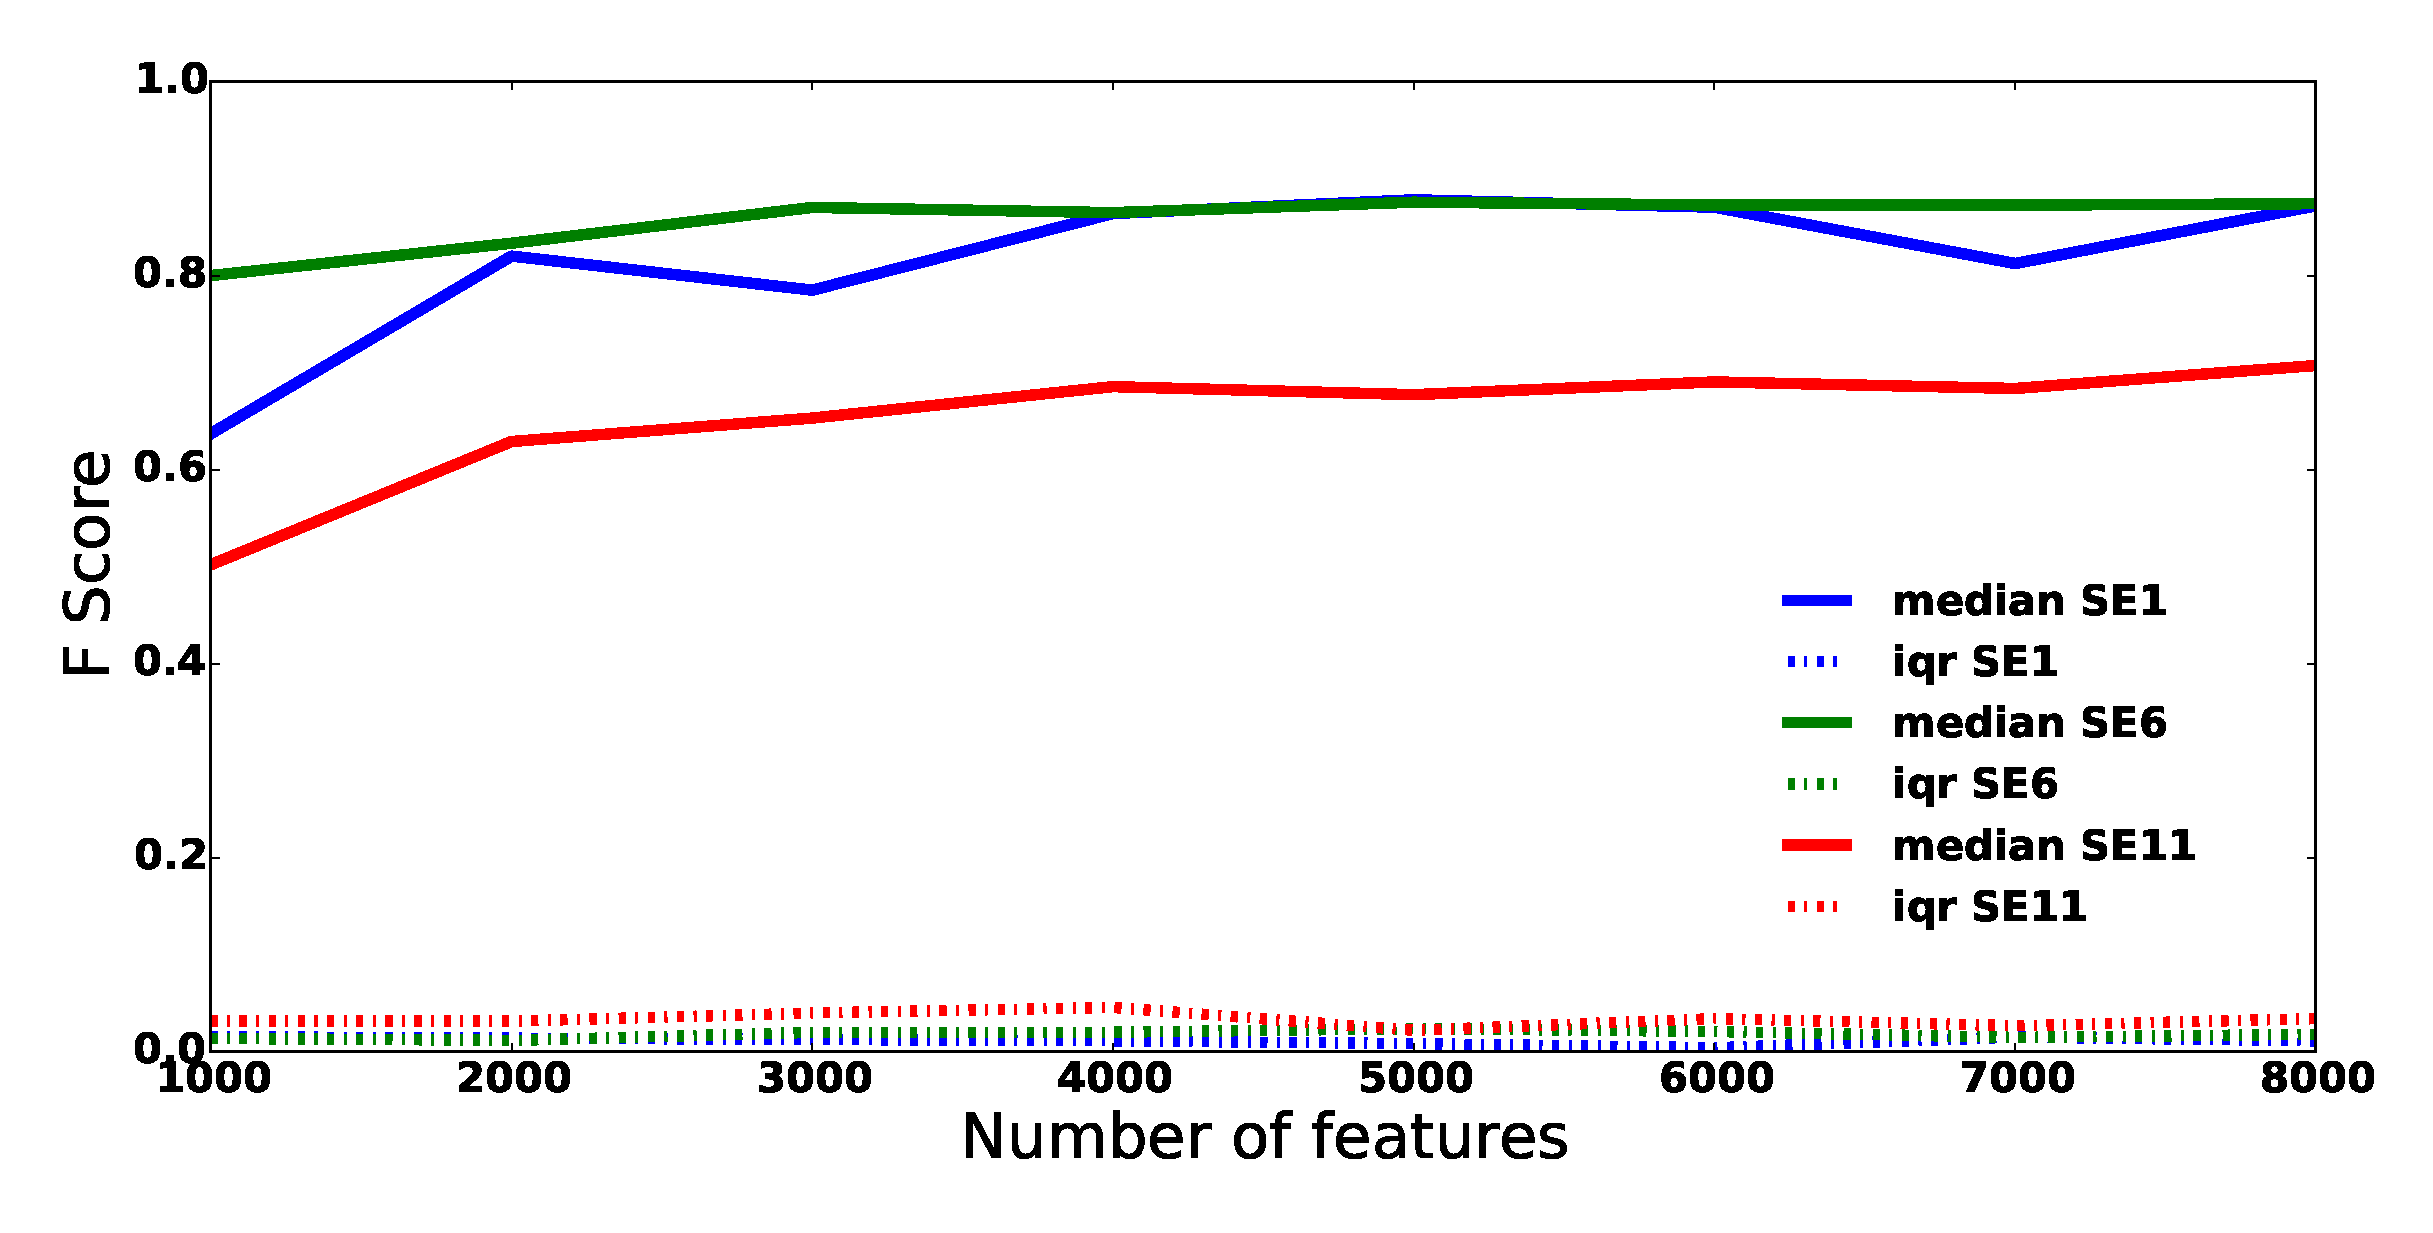
\includegraphics[width=\linewidth]{./fig/fea_num.eps}
%   \caption{Feature Numbers}
%   \label{fig:fea_num}
% \end{figure}


\subsubsection{Normalization}

Normalization is the process which adjust the values measured on different scales to a notionally common scale.

\textbf{Normalization on columns} transforms a  value $x$ in a column to $(x - \mathit{min})/(\mathit{max} - \mathit{min})$ (where $\mathit{min}$, $\mathit{max}$ come
from that column).
 In general data mining tasks, the weight of different features are measured on different scales. Normalization on columns of the feature matrix eliminates these differences among features. 

\textbf{L2 Normalization on rows} takes feature vector of each document and divide it by its L2 norm. It is the standard normalization method for text categorization \cite{frank2006naive}. The main purpose of implementing L2 normalization on rows is to rescale the vector of feature weights to unit length. 
For example, if results of applying the hashing
trick are {\em \{3, 3, 1\}}, then L2-normalization would divide each number by
$\sqrt{(3^2+3^2+1^2)}$ to produce $\{0.69,   0.69, 0.23\}$.
 

% \begin{figure}[ht]
%   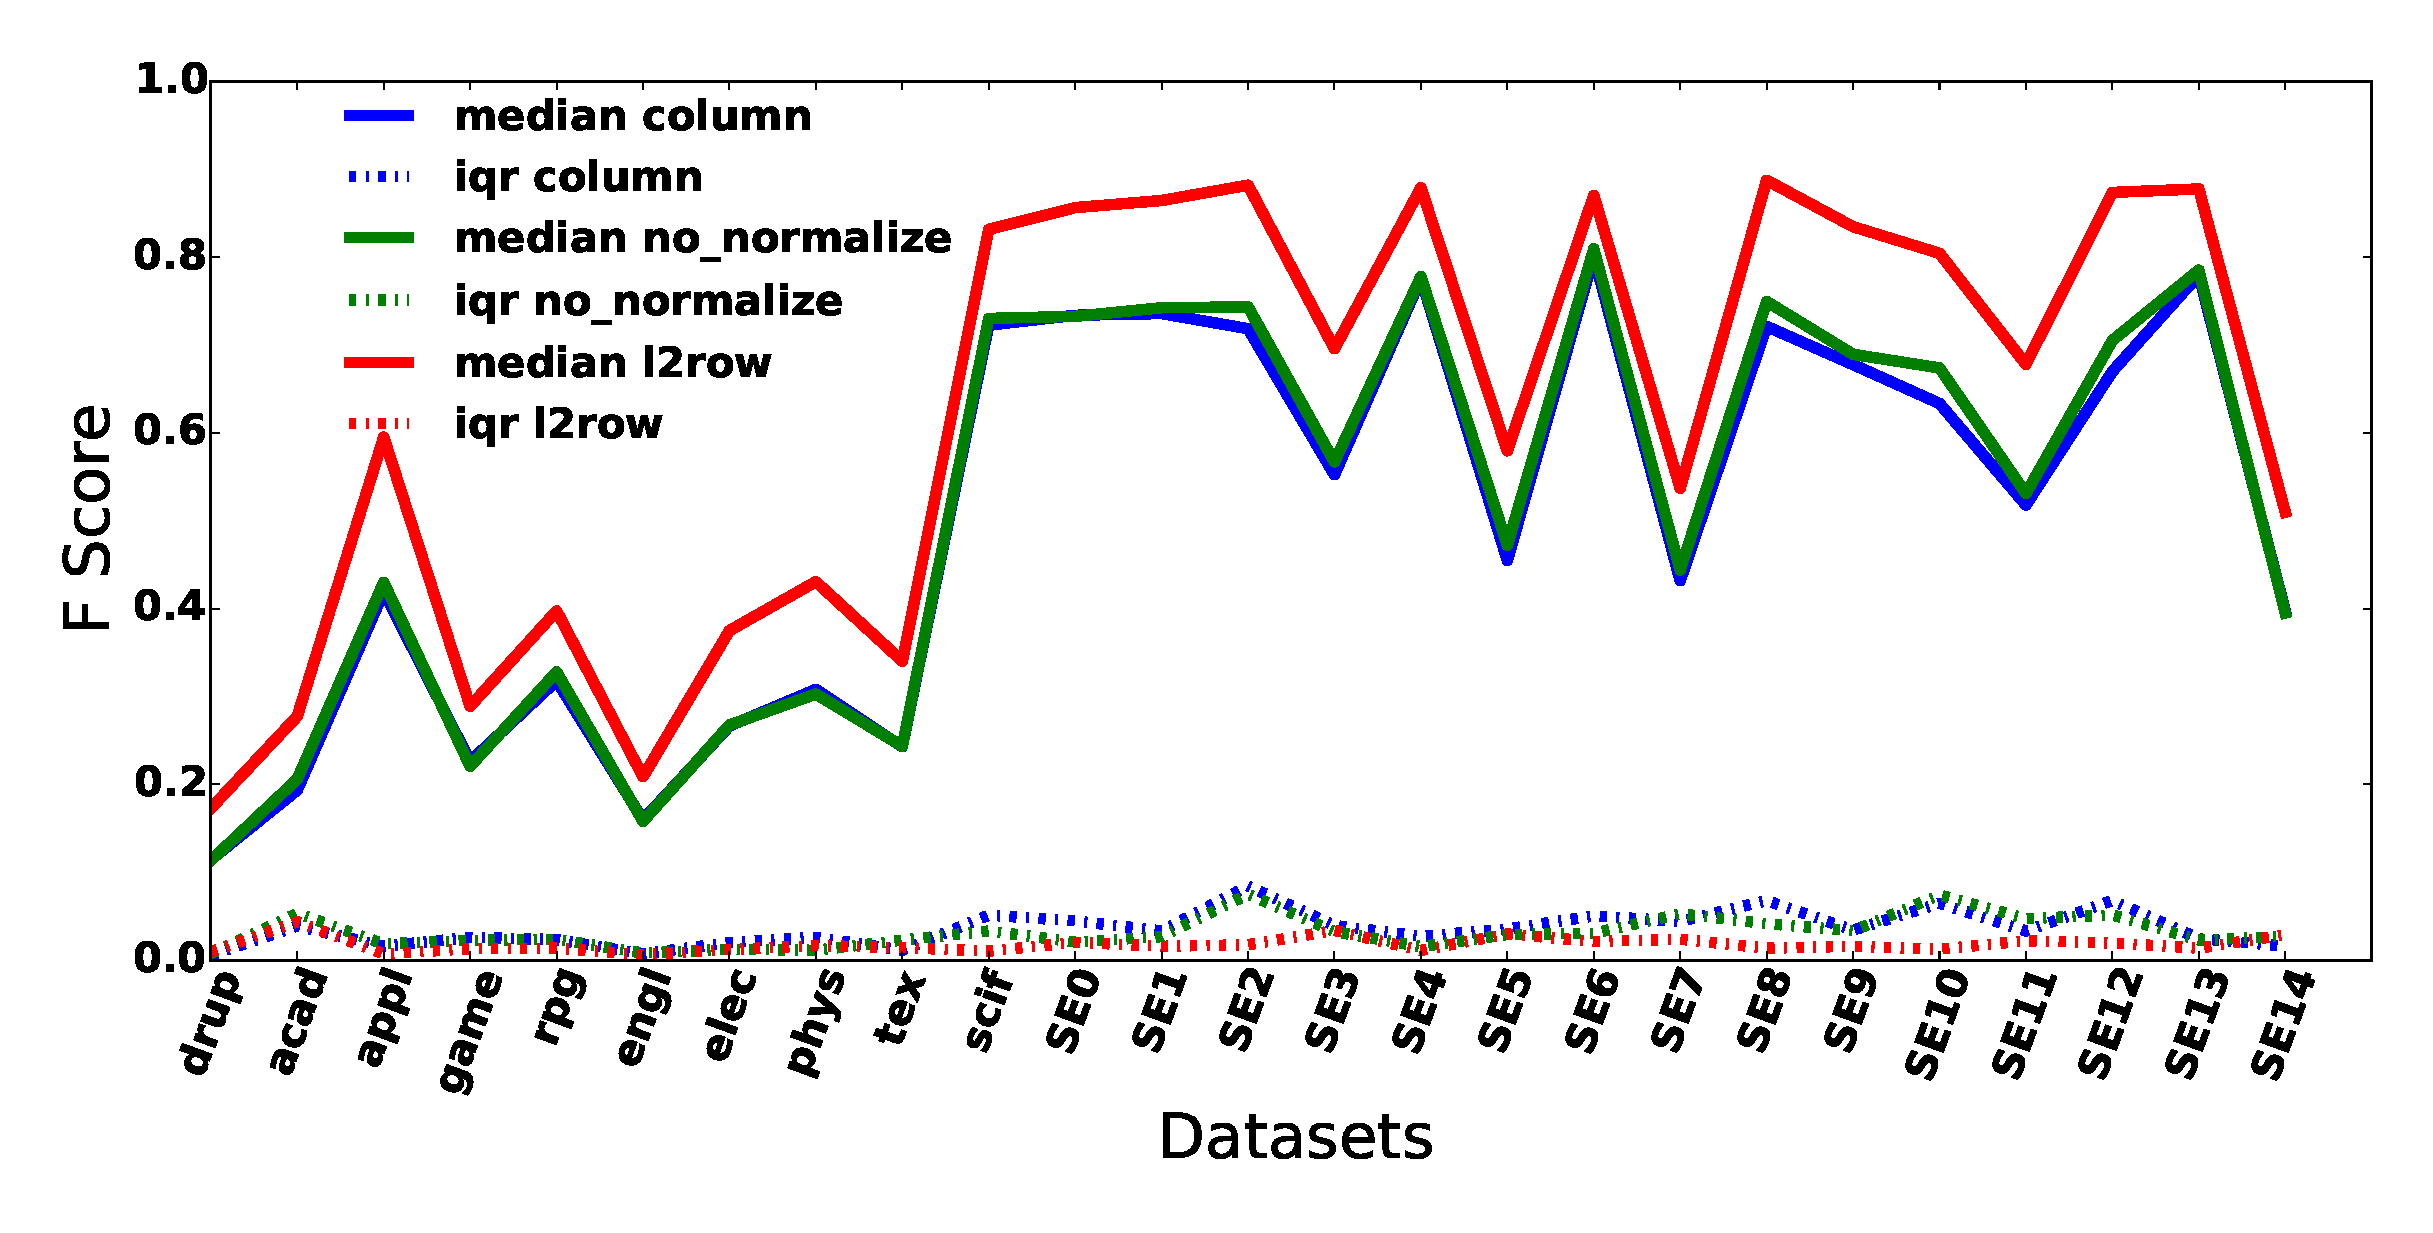
\includegraphics[width=\linewidth]{./fig/norm.eps}
%   \caption{Normalization methods}
%   \label{fig:norm}
% \end{figure}
 
 

As shown in Figure \ref{fig:norm}, column normalization offers little to no improvement
over no normalization. However, L2 Normalization on rows can add up to 20\% of the $F_1$ score.
\begin{lesson}
Normalizing rows can be more useful than normalizing columns.
\end{lesson}


\subsubsection{Data Balancing}
\label{sect:Data Balancing}

In imbalanced data sets, the target class are a small minority within the data.
The LexisNexis data is highly imbalanced with the target class may be as low as 2\% of the
data. Yet prior to BigSE, LexisNexis was not exploring data balancing methods.

Figure \ref{fig:balance} shows  experiments with applying the \textbf{SMOTE} data
balancer to our data.
 SMOTE over-samples the minority class by introducing synthetic examples along the line segments joining any pair of nearby real samples in neighborhood.  Proposed in 2002 \cite{chawla2002smote}, SMOTE is a very effective over-sampling method and has been widely applied during the past decades \cite{han2005borderline,bunkhumpornpat2009safe,luengo2011addressing}. 

% \begin{figure}[ht]
%   \includegraphics[width=\linewidth]{./fig/balance.eps}
%   \caption{SMOTE or not}
%   \label{fig:balance}
% \end{figure}
 
As shown in Figure \ref{fig:balance}, the average improvement of SMOTE in median value is 22\% on tag-level data and 17\% of site-level data. Note that, in these SMOTE experiments,
we SMOTEd the training set but the distributions in test set were left ``as is'',
Also, the average IQR for that plot is  4\%,9\% on tag-level,site-level data; i.e. is much smaller than the median
improvement. Hence we say:
\begin{lesson}
Class balancing (e.g. with SMOTE) is very useful for this kind of text mining.
\end{lesson}


\subsubsection{Classification}

Classifier guesses new labels using models built from prior data.
\textbf{SVM} is a widely-used learning model for  many data mining 
tasks \cite{joachims2006training,moharanatag}. SVM's use
some {\em kernel} that maps the raw data into another space where the data might be more
separable. 
Linear SVM is of the simplest kernel function but others include polynomial,
radial bias, sigmoid, etc.
 
There are many other kinds of classifiers.
\textbf{Naive Bayes} represents a family of simple probabilistic classifiers which has been studied extensively since 1950s. Multinomial Naive Bayes is especially designed for text categorization \cite{mccallum1998comparison} and always considered as a baseline method for text categorization. 

\textbf{Decision Tree} learners are  a popular model for classification. CART is one implementation of decision tree learners that has been proved useful in prior text mining applications~\cite{miotto2005supporting}.

% \begin{figure}[ht]
%   \includegraphics[width=\linewidth]{./fig/algms1.eps}
%   \caption{Classifiers}
%   \label{fig:algms1}
% \end{figure}
 
Figure \ref{fig:algms1} compares linear SVM with other kinds
of classifiers. The results from that figure are very clear:
linear SVM out-performs Naive Byes and decision tree learning
(with CART).
 
Figure \ref{fig:algms2} studies the effect of different
kernel functions in SVM. Note that linear SVM is the clear winner.
\begin{lesson}
Linear SVM is the recommended classifier for site-level data.
\end{lesson}
 

% \begin{figure}[ht]
%   \includegraphics[width=\linewidth]{./fig/algms2.eps}
%   \caption{Kernels}
%   \label{fig:algms2}
% \end{figure}










\section{Conclusions}
\label{sect:Conclusions}



This paper has listed the lessons learned from one the BigSE LexisNexis/NcState partnership.
This lab has found that.
most  of the operator choices made by LexisNexis are
  demonstrably better than many other choices.
However,  in some cases, NcState found certain operators
much faster than others (e.g. required only a single pass
of the data).
Also, in one case, NcState showed that one operator (SMOTE) not currently
used by LexisNexis offered useful improvements in their text miners.
SMOTE is now scheduled for inclusion in the next release
of the LexisNexis tools.

More specifically, for the site-level problem that is relevant to
LexisNexis' E-Discovery problem, BigSE recommends the following:
\be
\item \textbf{Tokenization:} Stemming and removal of stop words were generally useful. Shingling offered no noticeable benefits. 
\item \textbf{Featurization:} Contrary to popular recommendation, term frequency (TF) proved to work just as well as using TF-IDF.
\item \textbf{Normalization:}  Use L2 normalization on the rows.
\item \textbf{Dimensionality Reduction:} Given how there is so little difference between hashing trick and TF-IDF, using  the hashing trick in place of TF-IDF offered an added benefit of needing fewer dimensions (and less memory) and taking less time (TF-IDF needs  two passes of the data);
the hashing trick can be applied on each row, in a single pass
of the data).
\item \textbf{Data Balancing:} The low prevalence of "interesting" class in the test collection was handled   well by SMOTE.
\item \textbf{Classification:}  It  was surprising to note that a simple Linear SVM outperformed other kernels.
\ee
As mentioned above,    we make no presumption that the above list of choices
  works best for all text mining applications (but it
  is a set of choices that work better than others,
  in our domain).   As for other domains, we would recommend that organizations
assemble their own validation team to find the best choices in those domains.

The LexisNexis/NcState collaboration has been useful
for both parties.
LexisNexis got to explore more  text mining operators while
NcState got to expose their research students to the
realities of real-world industrial data mining.
 Also, BigSE has proved to be a pathway from
research to employment (e.g. BigSE  students  will work as    summer interns at  LexisNexis). 
Based on  these results, LexisNexis management has extended the collaboration till the end of 2016 (and further work in 2017
and beyond is begin discussed).

As to future work, as mentioned  above, these studies have  explored only a small portion of the very large space of operators available in text mining.
Our next phase is to explore automatic tuning methods that can explore that large space.
In order to explore a larger decision space as well as avoiding local optimum, heuristic search algorithms such as differential evolution, GALE, and NSGA-II will be applied to tune the decisions for a better approach \cite{storn1997differential,krall2015gale,deb2002fast}. We are working on this to achieve both less number of comparisons and better solutions.

Another useful future direction is
active learning.
One constant challenge in the LexisNexis work is gaining access to labelled data. In theory,
active learning could reduce the cost of humans reading and classifying documents during E-Discovery.
For example  instead of 20\% of the data, only a thousand samples will be selected and then used for training. The performance of prediction will rely heavily on how representative the selected samples are, and active learning is the key method to achieve it \cite{tong2002support}. 









 

%
% The following two commands are all you need in the
% initial runs of your .tex file to
% produce the bibliography for the citations in your paper.
 \renewcommand{\baselinestretch}{0.9}
 
\balance
\bibliographystyle{abbrv}
\small
\bibliography{sigproc}
\renewcommand{\baselinestretch}{1}

 % sigproc.bib is the name of the Bibliography in this case
% You must have a proper ".bib" file
%  and remember to run:
% latex bibtex latex latex
% to resolve all references
%
% ACM needs 'a single self-contained file'!
%
\end{document}
